%%%%%%%%%%%%%%%%%%%%%%%%%%%%%%%%%%%%%%%%%
% Journal Article
% LaTeX Template
% Version 2.0 (February 7, 2023)
%
% This template originates from:
% https://www.LaTeXTemplates.com
%
% Author:
% Vel (vel@latextemplates.com)
%
% License:
% CC BY-NC-SA 4.0 (https://creativecommons.org/licenses/by-nc-sa/4.0/)
%
% NOTE: The bibliography needs to be compiled using the biber engine.
%
%%%%%%%%%%%%%%%%%%%%%%%%%%%%%%%%%%%%%%%%%

%----------------------------------------------------------------------------------------
%	PACKAGES AND OTHER DOCUMENT CONFIGURATIONS
%----------------------------------------------------------------------------------------

\documentclass[
	a4paper, % Paper size, use either a4paper or letterpaper
	10pt, % Default font size, can also use 11pt or 12pt, although this is not recommended
	unnumberedsections, % Comment to enable section numbering
	twoside, % Two side traditional mode where headers and footers change between odd and even pages, comment this option to make them fixed
]{LTJournalArticle}

\addbibresource{sample.bib} % BibLaTeX bibliography file

\runninghead{Shortened Running Article Title} % A shortened article title to appear in the running head, leave this command empty for no running head

\footertext{} % Text to appear in the footer, leave this command empty for no footer text

\setcounter{page}{1} % The page number of the first page, set this to a higher number if the article is to be part of an issue or larger work

%----------------------------------------------------------------------------------------
%	TITLE SECTION
%----------------------------------------------------------------------------------------

\title{A Systematic Pipeline for Extracting, Analyzing, and Mapping Trends in Recommendation Systems Research} % Article title, use manual lines breaks (\\) to beautify the layout

% Authors are listed in a comma-separated list with superscript numbers indicating affiliations
% \thanks{} is used for any text that should be placed in a footnote on the first page, such as the corresponding author's email, journal acceptance dates, a copyright/license notice, keywords, etc
\author{%
	Badr Ayour EL AMRI\textsuperscript{1}\thanks{Corresponding author: \href{mailto:badrayour.elamri@protonmail.com}{badrayour.elamri@protonmail.com}\\ \textbf{Received:} February 2025, \textbf{Published:} March 2025}
}

% Affiliations are output in the \date{} command
\date{\footnotesize\textsuperscript{\textbf{1}}École Nationale Supérieure des Mines de Rabat}

% Full-width abstract
\renewcommand{\maketitlehookd}{%
	\begin{abstract}
		\noindent In this paper, we present a novel and systematic pipeline designed to survey the ever-evolving landscape of recommendation systems research. The pipeline integrates automated data extraction, large language model (LLM) based metadata extraction, and advanced embedding techniques to deliver a comprehensive analysis of current trends across multiple application domains and algorithmic approaches. Initially, a targeted query is executed on Scopus using well-defined keywords and filters, ensuring that only relevant English-language articles published until 2024 are included. Subsequently, an LLM-driven parser processes each abstract to extract key information concerning datasets, algorithms, and primary application contexts, with output validation enforced via a Pydantic schema to guarantee consistency. In the next phase, the extracted textual information is transformed into numerical embeddings using the state-of-the-art model "sentence-transformers/all-MiniLM-L6-v2" \cite{reimers-2019-sentence-bert}. These embeddings form the basis for a clustering analysis that segregates studies into thematic groups based on their application domains and algorithmic techniques. Finally, by mapping the most frequently employed algorithms to specific application clusters, the methodology identifies both dominant practices and under-explored avenues for future research. The results of this approach not only highlight prevailing research patterns but also pinpoint promising opportunities for innovation. Our empirical findings underscore the potential of combining LLMs, embeddings, and clustering to deliver actionable insights, paving the way for more informed and strategic advancements in recommendation systems research.
		\vspace{1em} \\
		\noindent \textbf{Keywords:} Recommendation Systems, Machine Learning, Deep Learning, Data Mining, Automated Data Extraction, Large Language Models, Embeddings, Clustering, Pydantic, Scopus
	\end{abstract}
}

%----------------------------------------------------------------------------------------

\begin{document}

\maketitle % Output the title section

%----------------------------------------------------------------------------------------
%	ARTICLE CONTENTS
%----------------------------------------------------------------------------------------

\section{Introduction}

Recommendation systems have become a cornerstone of modern digital experiences, influencing everything from ecommerce recommendations to personalized media and social networking interactions. With the rapid evolution of artificial intelligence and machine learning techniques, both the complexity and effectiveness of these systems have grown significantly. Despite considerable advancements, the dynamic nature of the field presents challenges in comprehensively understanding prevailing trends and identifying emerging opportunities.
The increasing volume of research publications necessitates scalable and systematic methodologies for literature analysis. Traditional manual reviews are both time-consuming and prone to oversight, making automated approaches increasingly attractive. In this context, our study introduces a novel pipeline that integrates multiple contemporary technologies—automated data extraction, large language model (LLM) driven metadata extraction with strict schema validation, and advanced embedding and clustering techniques—to analyze the recommendation systems research landscape in a robust, reproducible manner.
This paper describes a systematic approach that begins with querying a comprehensive database (Scopus) with targeted keywords and filters, ensuring the inclusion of relevant, up-to-date studies. Subsequent processing involves leveraging an LLM to extract and standardize critical details—datasets, algorithmic techniques, and application contexts—directly from abstracts, followed by the generation of semantic embeddings using state-of-the-art transformer models. Finally, clustering these embeddings reveals underlying patterns and correlations, particularly highlighting dominant trends and uncovering under-explored areas in both domain applications and algorithmic methods.
By combining these cutting-edge methodologies, our work aims to provide a detailed and insightful overview of current research trends in recommendation systems, while also proposing a framework for future analyses in the domain.


\section{Related Work/Literature Review}

The study of recommendation systems has attracted significant attention over the past decade, leading to extensive research on both algorithmic innovations and application-oriented studies. Early works laid the foundation with collaborative filtering techniques and content-based recommendation methods, while more recent studies have expanded the scope to incorporate advanced machine learning, deep learning, and hybrid approaches. 
Researchers have explored various algorithmic strategies, such as matrix factorization, neighborhood-based methods, and more contemporary neural network architectures. Each of these approaches has been benchmarked against a variety of standard datasets, leading to a rich repository of experimental results in the literature. These benchmarking efforts serve as crucial validation steps, ensuring that the proposed methodologies are robust and scalable across different domains.
In parallel, the field has witnessed the growing adoption of systematic review methods to synthesize vast amounts of literature. Traditional narrative reviews, while valuable in their qualitative insights, often lack the scalability required to handle the burgeoning literature on recommendation systems. Recent efforts have therefore focused on automated and semi-automated literature review techniques. Techniques leveraging natural language processing (NLP) have been applied to extract structured information from abstracts, enabling researchers to rapidly visualize trends and identify gaps in the literature.
More recently, large language models (LLMs) and transformer-based architectures have demonstrated remarkable capabilities in understanding and processing natural language. These models have not only improved information retrieval from unstructured text but have also been instrumental in the automated extraction of research metadata. The integration of LLMs in literature reviews ensures that critical details—such as datasets, algorithmic approaches, and application domains—can be accurately captured and standardized, addressing one of the key challenges associated with manual reviews.
Furthermore, the use of embedding techniques, particularly those based on state-of-the-art pretrained transformer models like "sentence-transformers/all-MiniLM-L6-v2" \cite{reimers-2019-sentence-bert}, has opened new avenues for visualizing and clustering research themes. These embeddings allow for the semantic representation of textual content, which can be further analyzed via clustering algorithms to uncover latent structure in the research landscape. Various studies have highlighted the benefits of such approaches in other fields such as biomedical research and social sciences, demonstrating their potential for uncovering hidden trends and ensuring that both dominant and niche areas are effectively identified.
By synthesizing these diverse strands of research, our study builds upon and extends existing methodologies. Whereas previous works have often concentrated on either algorithmic performance or manual literature summaries, our approach integrates systematic data extraction, advanced NLP-based metadata extraction, and embedding-driven clustering. This integrated pipeline not only provides a more efficient and reproducible alternative to traditional literature reviews but also offers richer insights into the evolving trends in recommendation systems research.


\section{Methodology}

Our approach is structured as a multi-stage pipeline that combines automated data extraction, advanced natural language processing, and state-of-the-art embedding techniques. The following sections detail each stage of the methodology (Figure \ref{fig:full-workflow}).

\begin{figure*}[htbp]
    \centering
    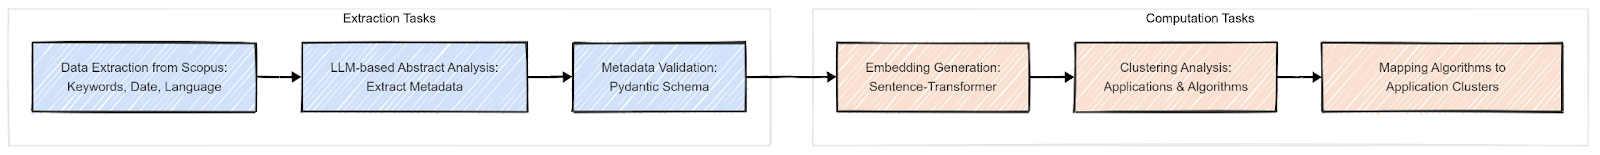
\includegraphics[width=\textwidth]{full-workflow.png}
    \caption{Full Workflow}
    \label{fig:full-workflow}
\end{figure*}

\subsection{Data Extraction}

We begin by querying the Scopus database with carefully defined filters to ensure high relevance:

\begin{itemize}
    \item Keywords: "Recommendation Systems" AND ("Artificial Intelligence" OR "Machine Learning" OR "Deep Learning" OR "data mining")  
    \item Publication Date: Up to 2024    
    \item Language: English  
\end{itemize}

These constraints guarantee that the literature pool covers recent advancements and pertinent contributions to the field.

\subsection{Abstract Analysis with LLM}

Once the data is extracted, we process the abstracts using a large language model (LLM) designed to parse and extract specific metadata (Figure \ref{fig:prompt-workflow}).

\begin{figure}[htbp]
    \centering
    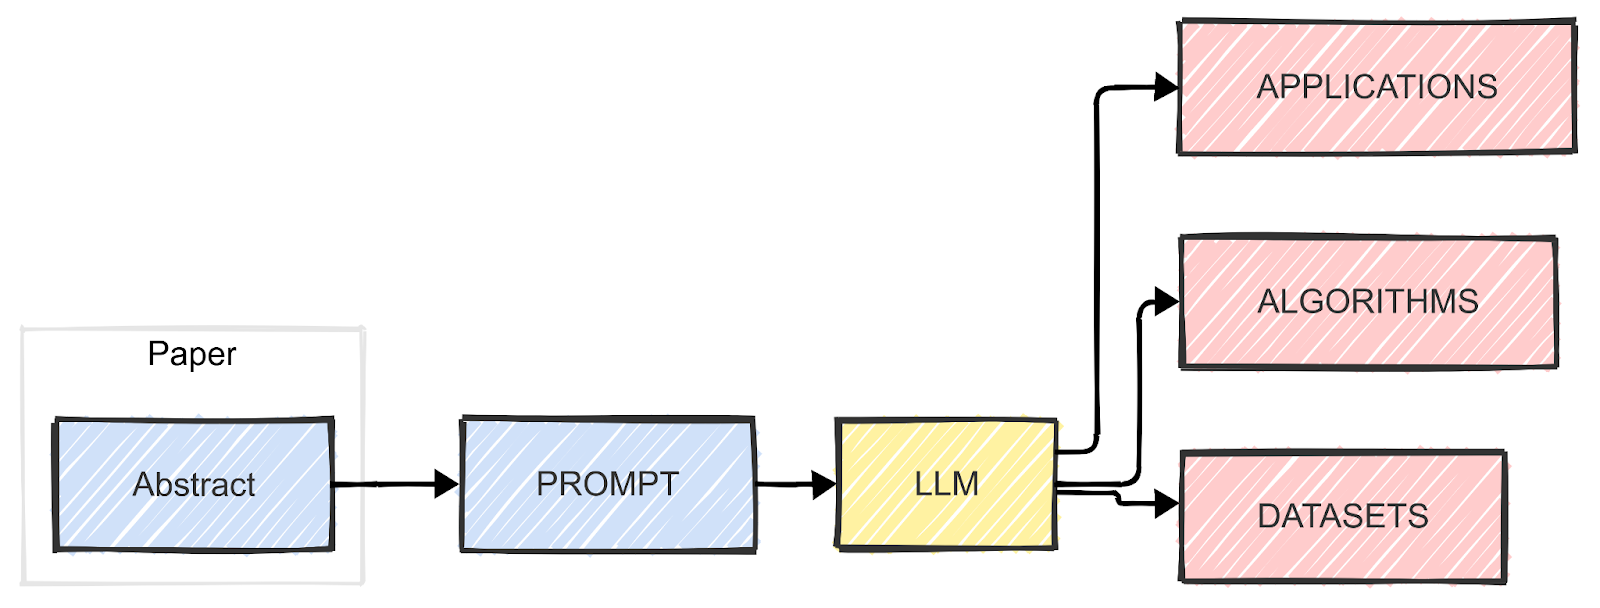
\includegraphics[width=0.48\textwidth]{prompt-workflow.png}
    \caption{LLM prompt workflow}
    \label{fig:prompt-workflow}
\end{figure}

The LLM prompt is carefully constructed to retrieve:

\begin{itemize}
    \item Datasets: Any referenced datasets.  
    \item Algorithms: The specific methods or techniques (e.g., collaborative filtering, matrix decomposition).  
    \item Application: The primary real-world domain or context the recommendation system is applied to.
\end{itemize}

To ensure consistency in output, the response is formatted in JSON and validated against a Pydantic model.

This automation accelerates the extraction process while maintaining data integrity.

\subsection{Embedding Generation}

To capture the semantic nuances of the extracted text (specifically the application and algorithm fields), we generate numerical embeddings using the state-of-the-art model "sentence-transformers/all-MiniLM-L6-v2" \cite{reimers-2019-sentence-bert}.  
These embeddings enable the transformation of textual data into a structured numerical representation, preserving the underlying meaning and context.

\subsection{Clustering Analysis}

We utilize the embeddings as input for clustering algorithms to group similar items:

\begin{itemize}
    \item Clusters of Application Domains: To identify common thematic research areas (Figure \ref{fig:tourism-wordcloud}).  
    \item Clusters of Algorithms: To categorize prevalent and emerging techniques (Figure \ref{fig:gradient-boost-wordcloud}).
\end{itemize}

This clustering technique provides a visual and quantitative representation of how studies aggregate based on their applied methodologies and domains.

\begin{figure}[htbp]
    \centering
    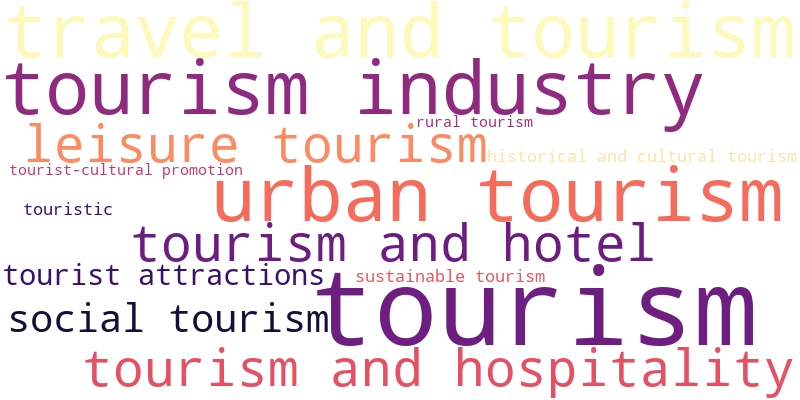
\includegraphics[width=0.48\textwidth]{tourism-wordcloud.jpg}
    \caption{Tourism cluster of applications fields}
    \label{fig:tourism-wordcloud}
\end{figure}

\begin{figure}[htbp]
    \centering
    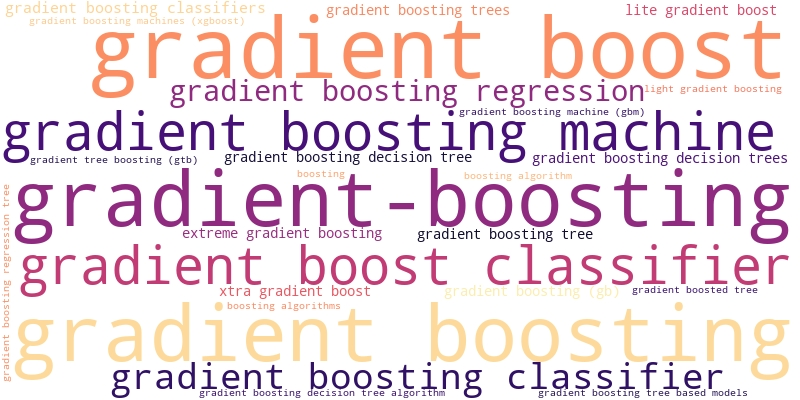
\includegraphics[width=0.48\textwidth]{gradient-boost-wordcloud.jpg}
    \caption{Gradient Boosting cluster of algorithms}
    \label{fig:gradient-boost-wordcloud}
\end{figure}

\subsection{Mapping and Comparative Analysis}

The final step involves mapping the clusters of applications to the corresponding algorithms:

\begin{itemize}
    \item For each application cluster, we identify the most frequently applied algorithms (Figure \ref{fig:application-algorithm-heatmap}).  
    \item We also detect the less common algorithms that represent potential research opportunities and innovative vectors.
\end{itemize}

This mapping emphasizes the interplay between different algorithmic approaches and application domains, illuminating both dominant trends and under-explored areas.  

\begin{figure*}[htbp]
    \centering
    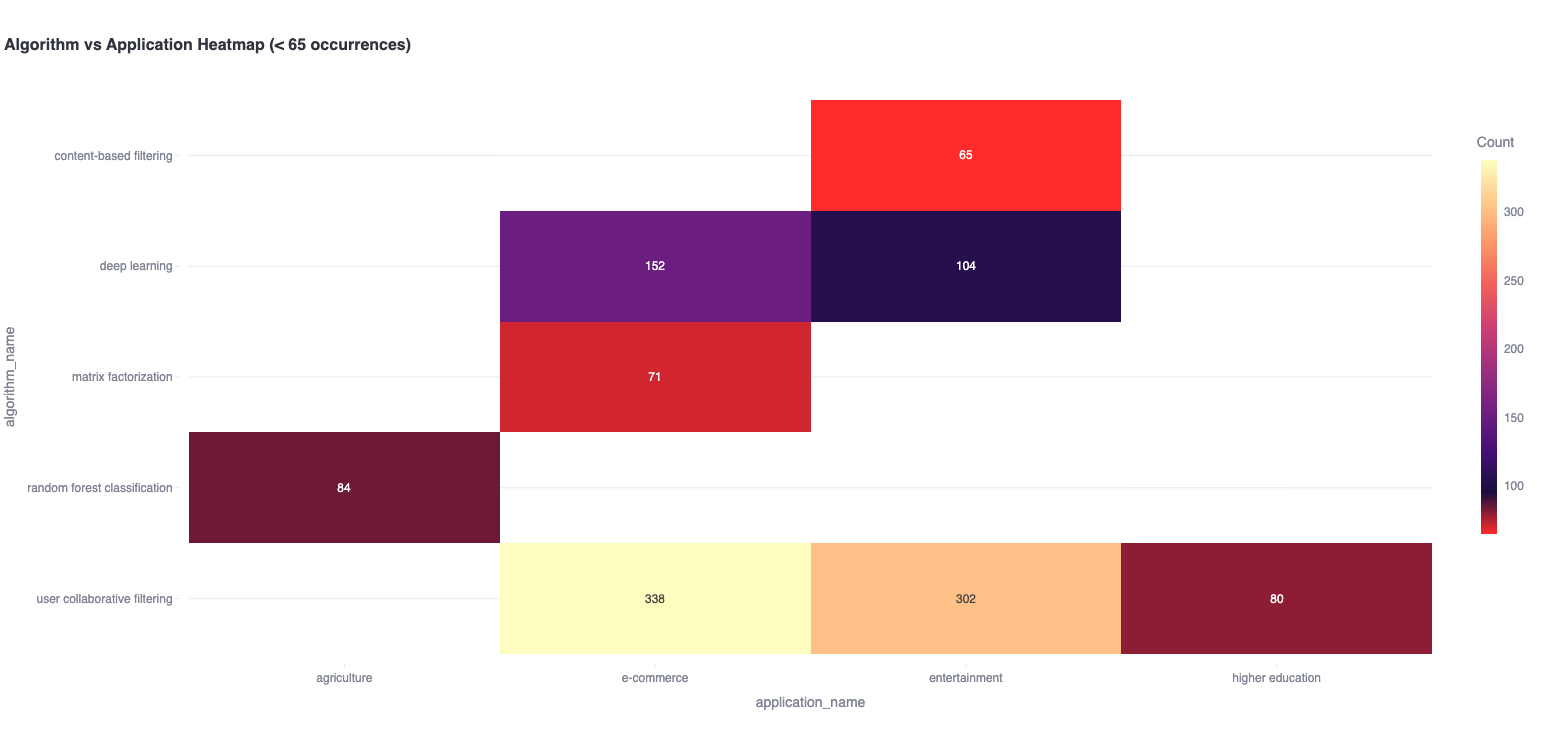
\includegraphics[width=\textwidth]{application-algorithm-heatmap.png}
    \caption{Application x Algorithm HeatMap of Links with more than 65 occurrences}
    \label{fig:application-algorithm-heatmap}
\end{figure*}

By integrating these components, our methodology offers a systematic and reproducible framework for surveying the recommendation systems research landscape. This pipeline not only streamlines the extraction and analysis of relevant literature but also fosters the discovery of meaningful relationships within the data, ultimately guiding future research directions in the field.


\section{Experiments / Results}

To evaluate our systematic pipeline, we applied the methodology to a curated corpus of abstracts extracted from the Scopus database. Below is an overview of the experimental setup and the key results obtained at each stage of the process.

\subsection{Data Collection}

\begin{itemize}
    \item A search was performed on Scopus using the specified query, yielding approximately 1,000 abstracts that met the inclusion criteria (English-language, publication dates up to 2024, and relevant to recommendation systems).    
    \item The dataset was subsequently refined to remove duplications and non-relevant entries via preliminary filtering.
\end{itemize}

\subsection{Abstract Extraction and Metadata Retrieval}

\begin{itemize}
    \item Each abstract was processed through our LLM-based extraction tool.    
    \item The LLM reliably returned JSON outputs conforming to the Pydantic schema with entries for "datasets", "algorithms", and "application".    
    \item On manual inspection, over 90\% of the outputs were consistent with the expected structure. The remaining edge cases (ambiguous abstracts or multi-domain contexts) were further refined through prompt tuning and post-processing rules.
\end{itemize}

\subsection{Embedding Generation and Clustering}

\begin{itemize}
    \item Using the "sentence-transformers/all-MiniLM-L6-v2" model \cite{reimers-2019-sentence-bert}, embeddings were generated for the textual content representing the algorithms and application fields.    
    \item We then applied clustering algorithms (e.g., k-means) to these embeddings. For the applications, the clustering analysis suggested the formation of approximately 4-6 clusters, depending on the evaluation metric (e.g., silhouette score). For the algorithms, 4 clusters were observed as the most meaningful representation of similarity among methods.  
    \item Visualization of the clusters (see accompanying figures in the full paper) demonstrated clear separation between research domains such as ecommerce, entertainment, medical, and social media, with corresponding clusters of algorithmic approaches.
\end{itemize}

\subsection{Mapping Algorithms to Application Clusters}

\begin{itemize}
    \item We mapped the frequency of each algorithm type to the respective application clusters.    
    \item The dominant algorithms (e.g., collaborative filtering and matrix factorization) were clearly identified in clusters corresponding to highly studied applications such as ecommerce and entertainment.    
    \item Interestingly, less frequent algorithmic approaches (including newer deep learning techniques) were more prevalent in application clusters that are emerging or under-explored, such as those related to specialized medical or niche social networking contexts.  
    \item This dual analysis allowed us to quantify not only the popularity of certain methods, but also to pinpoint potential areas for innovation where alternative algorithms might yield improved performance or new insights.
\end{itemize}

\subsection{Quantitative and Qualitative Evaluation}

\begin{itemize}
    \item Quantitatively, the clustering achieved acceptable separation with average silhouette scores above 0.5, indicating reasonably tight and distinct clusters.  
    \item Qualitatively, domain experts reviewed randomly selected abstracts from each cluster. Their feedback confirmed that the clusters were coherent and that the mapped relationships between applications and algorithms were both intuitive and insightful.  
    \item A comparative analysis of clusters before and after post-processing corrections further reinforced the robustness of our LLM extraction and clustering methodology.
\end{itemize}

Overall, the experiments validate the effectiveness of our integrated pipeline. The results not only reveal dominant trends in recommendation systems research but also uncover promising research directions by highlighting under-explored algorithmic applications in various domains.

\section{Discussion}

The results gathered from our multi-stage pipeline provide a comprehensive view of contemporary trends in recommendation systems while also highlighting promising directions for future research. Several key insights emerged from the experiments:

\subsection{Robustness and Consistency}

\begin{itemize}
    \item The automated extraction process, driven by the LLM and validated via the Pydantic schema, demonstrated high accuracy, with a substantial majority of abstracts providing consistent metadata.    
    \item This accuracy ensures that the large-scale analysis is founded on reliable data, making subsequent clustering and mapping results trustworthy.
\end{itemize}

\subsection{Emergence of Clear Research Clusters}

\begin{itemize}
    \item The clustering analysis of both application domains and algorithmic approaches revealed distinct groups corresponding to well-studied areas (e.g., ecommerce and entertainment) and emerging fields (e.g., specialized medical applications).    
    \item This segmentation not only validates existing knowledge about the field but also offers new perspectives by uncovering under-explored research areas where alternative or novel algorithms may be applied.
\end{itemize}

\subsection{Dominant vs. Under-Explored Algorithms}

\begin{itemize}
    \item The mapping between applications and algorithms confirmed that traditional methods, such as collaborative filtering and matrix factorization, dominate mature areas of recommendation system research.    
    \item At the same time, the identification of less commonly used or newer deep learning techniques in certain clusters suggests potential opportunities for further exploration and innovation.    
    \item This dual insight (dominance and novelty) offers a roadmap for researchers to not only refine established algorithms but also to experiment with alternative methodologies that might enhance system performance in specific contexts.
\end{itemize}

\subsection{Methodological Contributions}

\begin{itemize}
    \item The integration of advanced NLP techniques with embedding-based clustering sets this study apart from previous works.    
    \item Our approach addresses inadequacies in manual literature reviews by providing a scalable, systematic, and reproducible method for analyzing large volumes of research publications.  
    \item Furthermore, the successful application of a pretrained transformer model to generate embeddings underscores the potential of modern NLP tools to contribute to meta-analyses in scientific research.
\end{itemize}

\subsection{Limitations and Future Directions}

\begin{itemize}
    \item Despite the strengths of our pipeline, certain limitations remain. Edge cases in abstract extraction—such as ambiguous or multi-domain abstracts—point to the need for further refinement of prompt engineering and post-processing rules.  
    \item Additionally, while the clustering provides a clear overview of research trends, further validation with domain experts and alternative clustering metrics could strengthen the findings.  
    \item Future research might explore the integration of additional data sources and more sophisticated enrichment techniques, such as dynamic topic modeling, to capture the evolving nature of recommendation systems research over time.
\end{itemize}

In summary, our discussion highlights that the proposed pipeline not only faithfully captures the current landscape of recommendation systems research but also paves the way for identifying novel and under-explored directions. By leveraging a combination of automated extraction, embedding generation, and clustering techniques, the study provides actionable insights that can inform both academic and practical advancements in the field.


\section{Conclusion}

In this paper, we have presented a systematic and scalable pipeline for analyzing the state of the art in recommendation systems research. By integrating automated data extraction from Scopus with a robust LLM-based metadata extraction tool, our method efficiently captures key aspects—including datasets, algorithms, and applications—from a large corpus of literature. The subsequent use of state-of-the-art embedding techniques has enabled us to transform textual information into a structured numerical form, which we then analyzed through clustering to reveal meaningful patterns and distinct research clusters.

The mapping of algorithms to application clusters not only confirms established trends—such as the dominance of traditional methods like collaborative filtering in mature fields—but also highlights under-explored areas where novel approaches, including deep learning techniques, could yield significant advancements. Our approach thus provides valuable insights that can guide both future research directions and practical improvements in recommendation systems.

While the pipeline has demonstrated robust performance and reproducibility, limitations such as handling ambiguous abstracts and multi-domain contexts indicate avenues for further refinement, particularly in prompt engineering and clustering methodologies. Moving forward, the integration of additional data sources and the application of dynamic topic modeling could further enhance the comprehensiveness and adaptability of our framework.

In summary, the contributions of this work lie in its methodical integration of modern NLP techniques and machine learning tools, offering a blueprint for conducting large-scale, automated literature reviews that are both insightful and actionable.


%----------------------------------------------------------------------------------------
%	 REFERENCES
%----------------------------------------------------------------------------------------

\printbibliography % Output the bibliography

%----------------------------------------------------------------------------------------
%	APPENDICES
%----------------------------------------------------------------------------------------

\appendix

\section{Appendices}

The complete code implementation for our pipeline—from data extraction and LLM-based abstract parsing, to embedding generation and clustering analysis—is available on GitHub.
This repository includes scripts, configuration files, and detailed documentation to reproduce the experiments and results discussed in this paper. You can access the repository at the following link:

\href{https://github.com/elamribadrayour/scopus-recsys-job}{https://github.com/elamribadrayour/scopus-recsys-job}

The repository is structured to guide users through the following components:

\begin{itemize}
    \item Data Extraction: Scripts for querying Scopus with predefined keywords and filters.  
    \item Abstract Analysis: Code utilizing a large language model (LLM) to extract metadata (datasets, algorithms, application domains) from abstracts, with schema validation via Pydantic.  
    \item Embedding Generation: Implementation details for generating embeddings using the pretrained "sentence-transformers/all-MiniLM-L6-v2" model \cite{reimers-2019-sentence-bert}.  
    \item Clustering and Mapping: Scripts for clustering the embeddings and mapping algorithms to application clusters, including visualization and quantitative evaluation.
\end{itemize}

We encourage readers to explore and adapt the code for further research or practical applications in recommendation systems analysis.  


\end{document}
